% !TEX program = xelatex
% Kompilacja (minted wymaga -shell-escape):
%   latexmk -xelatex -shell-escape sprawozdanie-koncowe.tex
%   lub przez Taskfile:  task report
\documentclass[11pt,a4paper]{article}

% ------------------------------------------------------------------
%  Pakiety podstawowe (XeLaTeX + język polski)
% ------------------------------------------------------------------
\usepackage{fontspec}
\usepackage{polyglossia}
\setdefaultlanguage{polish}
\setmainfont{Latin Modern Roman}
\setsansfont{Latin Modern Sans}
\setmonofont{Latin Modern Mono}

\usepackage[a4paper,margin=2.4cm]{geometry}
\usepackage{amsmath}
\usepackage{microtype}
\usepackage{graphicx}
\usepackage{booktabs}
\usepackage{enumitem}
\usepackage{xcolor}
\usepackage[newfloat]{minted}
\usepackage{caption}
\usepackage{float}
\usepackage{rotating}
\usepackage{hyperref}

\hypersetup{
  colorlinks=true,
  linkcolor=black,
  urlcolor=blue!60!black,
  citecolor=black,
  pdftitle={Sprawozdanie końcowe - Password Break},
  pdfauthor={Rafał Grot, Dominika Jedynak, Kacper Kaczmarczyk}
}

% ------------------------------------------------------------------
%  TikZ - diagramy generowane przy kompilacji
% ------------------------------------------------------------------
\usepackage{tikz}
\usetikzlibrary{positioning,arrows.meta,shapes.multipart,shapes.geometric,fit,calc,backgrounds}

% Kolory
\definecolor{srvcol}{RGB}{31,119,180}
\definecolor{clicol}{RGB}{214,96,30}
\definecolor{moncol}{RGB}{44,140,80}
\definecolor{boxbg}{RGB}{240,244,250}
\definecolor{codebg}{RGB}{246,246,246}

% Styl bloków UML (rectangle split: nazwa / pola / metody)
\tikzset{
  umlclass/.style={
    rectangle split, rectangle split parts=3, draw=black!70, thick,
    rectangle split draw splits=true, fill=boxbg, align=left,
    text width=46mm, font=\footnotesize, inner sep=2pt,
    rectangle split part align=left
  },
  umlclass2/.style={
    rectangle split, rectangle split parts=2, draw=black!70, thick,
    rectangle split draw splits=true, fill=boxbg, align=left,
    text width=46mm, font=\footnotesize, inner sep=2pt,
    rectangle split part align=left
  },
  comp/.style={rectangle, rounded corners, draw=black!70, thick, fill=boxbg,
    align=center, minimum height=12mm, minimum width=30mm, font=\small},
  arr/.style={-{Stealth[length=2.4mm]}, thick},
  darr/.style={{Stealth[length=2.4mm]}-{Stealth[length=2.4mm]}, thick},
}

% ------------------------------------------------------------------
%  Styl fragmentów kodu (minted -> wymaga kompilacji z -shell-escape)
% ------------------------------------------------------------------
\setminted{
  fontsize=\scriptsize,
  bgcolor=codebg,
  breaklines=true,
  breakanywhere=true,
  frame=single,
  framesep=4pt,
  tabsize=2,
}
\setmintedinline{fontsize=\normalsize}
% nazwijmy pływające listingi „Listing”
\SetupFloatingEnvironment{listing}{name=Listing}

\captionsetup{font=small,labelfont=bf}
\setlist{topsep=2pt,itemsep=1pt,parsep=0pt}

\title{Sprawozdanie końcowe \\[0.3em] \large Password Break}
\author{Rafał Grot \and Dominika Jedynak \and Kacper Kaczmarczyk}
\date{\the\year}

% ==================================================================
\begin{document}

\maketitle

\tableofcontents
\newpage

% ==================================================================
\section{Wstęp}

\subsection{Charakterystyka problemu}
Hasła w rzeczywistych systemach nie są przechowywane w postaci jawnej, lecz jako wynik
działania kryptograficznej funkcji skrótu. System uwierzytelniający nie zna bezpośrednio
tekstu hasła, a jedynie jego skrót. Projektowany program nie odwraca funkcji haszującej (co
jest obliczeniowo niewykonalne), lecz \emph{generuje} kolejnych kandydatów na hasło, oblicza ich
skróty i porównuje je ze skrótem docelowym.

Problem można rozproszyć na wiele komputerów: poszczególni klienci niezależnie sprawdzają
różne fragmenty przestrzeni możliwych haseł, a serwer przydziela pracę i zbiera wyniki.
Sprawdzanie kolejnych haseł nie zależy od siebie nawzajem, więc obliczenia różnych klientów
nie wymagają wzajemnej synchronizacji.

\subsection{Cel projektu}
Celem projektu jest zbudowanie działającego systemu rozproszonego i analiza jego wydajności
przy różnych konfiguracjach pracy. System obejmuje:
\begin{itemize}
  \item komunikację klient--serwer w trybie dwukierunkowego strumienia,
  \item dynamiczny przydział i synchronizację pracy,
  \item obsługę błędów (rozłączenia, zawieszenia klientów, ponowny przydział zadań),
  \item pomiar i analizę wydajności (przepustowość, skalowalność, wpływ granulacji).
\end{itemize}

Mierzone są między innymi: liczba sprawdzonych kandydatów na sekundę, wpływ liczby klientów
na wydajność, wpływ granulacji (wielkości paczek zadań) oraz narzut komunikacji względem
czasu właściwych obliczeń.

\subsection{Podstawy teoretyczne}

\paragraph{Funkcja skrótu SHA-256.}
SHA-256 przekształca dane wejściowe dowolnej długości w ciąg o stałej długości 256 bitów
(32 bajty). Kluczowe właściwości wykorzystywane w projekcie to:
\begin{itemize}
  \item \emph{deterministyczność}, te same dane zawsze dają ten sam skrót,
  \item \emph{jednokierunkowość}, nie da się praktycznie odtworzyć danych ze skrótu,
  \item \emph{odporność na kolizje} oraz \emph{efekt lawinowy}, minimalna zmiana wejścia
        całkowicie zmienia skrót.
\end{itemize}
Najdroższą operacją jest samo haszowanie, dlatego opłaca się porównywać jeden skrót z wieloma
kandydatami, a target hashe trzymać w strukturze \texttt{HashSet} o stałym czasie wyszukiwania.

\paragraph{Atak brute force.}
Metoda generuje wszystkie możliwe kombinacje znaków z ustalonego alfabetu (małe litery,
cyfry, ewentualnie znaki specjalne) w zadanym zakresie długości. Jest pewna, ale kosztowna
obliczeniowo. Aby podzielić pracę, wszystkie możliwe hasła zostają \emph{ponumerowane}, a serwer
przydziela klientom zakresy indeksów do sprawdzenia (patrz rozdz.~\ref{sec:bf-index}).

\paragraph{Atak słownikowy.}
Metoda sprawdza hasła z przygotowanego pliku (słownika) zawierającego często spotykane słowa i
ich warianty (dodane cyfry, zmiana wielkości liter, znaki specjalne, podstawienia typu
\texttt{a}$\rightarrow$\texttt{@}, \texttt{o}$\rightarrow$\texttt{0}). Pozwala szybko znaleźć słabe
hasła. W systemie rozproszonym słownik dzielony jest na zakresy indeksów tak samo jak w trybie
brute force.

% ==================================================================
\section{Założenia projektowe}

\subsection{Zakres funkcjonalny}
\begin{itemize}
  \item Aplikacja serwera uruchamiana z konsoli, z parametrami zadania w pliku konfiguracyjnym.
  \item Aplikacja klienta uruchamiana z konsoli, z adresem serwera podawanym jako argument.
  \item Obsługa dwóch trybów pracy: \emph{brute force} oraz \emph{słownikowego}.
  \item Dynamiczny przydział paczek zadań klientom, którzy zgłoszą gotowość.
  \item Wielowątkowe obliczenia po stronie klienta.
  \item Logowanie wyników oraz metryk wydajności do plików CSV po stronie serwera.
  \item Możliwość uruchamiania na różnej liczbie klientów (skalowanie poziome).
\end{itemize}

\subsection{Przypadki użycia}
\begin{enumerate}
  \item Użytkownik uruchamia serwer i ustawia parametry zadania (tryb, alfabet, długości, skróty docelowe).
  \item Użytkownik uruchamia klientów na kolejnych komputerach, wskazując adres serwera.
  \item Klient łączy się, pobiera konfigurację i oczekuje na sygnał startu.
  \item Po starcie klient pobiera paczkę pracy, wykonuje obliczenia i odsyła wynik, po czym pobiera następną.
  \item Klient znajduje poprawne hasło i raportuje je do serwera.
  \item Serwer zapisuje końcowy raport i metryki testu.
\end{enumerate}

\subsection{Wybór technologii}
\begin{center}
\begin{tabular}{@{}ll@{}}
\toprule
\textbf{Obszar} & \textbf{Technologia} \\
\midrule
Platforma / język          & .NET, C\# \\
Komunikacja sieciowa       & gRPC (HTTP/2), Protocol Buffers (proto3) \\
Serwer                     & ASP.NET Core gRPC Service \\
Klient, generator, Plots   & aplikacje konsolowe .NET \\
Wykresy                    & ScottPlot \\
Środowisko        & Nix flake (dev-shell) \\
\bottomrule
\end{tabular}
\end{center}

W projekcie zastosowano architekturę klient--serwer: jeden węzeł pełni rolę koordynatora
(serwer), pozostałe wykonują obliczenia (klienci). gRPC wybrano jako nowsze rozwiązanie
oraz dlatego, że podejście \emph{contract-first} (wspólny plik \texttt{.proto}, z którego
generowany jest kod serwera i klienta) jest prostsze niż budowanie API w REST. Dodatkowo gRPC
ma wbudowaną obsługę strumieni dwukierunkowych, których ten system potrzebuje.

\subsection{Komponenty systemu}
Repozytorium zawiera rozwiązanie \texttt{password-break.slnx} złożone z następujących projektów:
\begin{description}[style=nextline,leftmargin=0pt]
  \item[\texttt{password-break-server}] Serwer koordynujący: dzieli przestrzeń przeszukiwania na
        zadania, przydziela je klientom, zbiera wyniki, mierzy i zapisuje metryki.
  \item[\texttt{password-break-client}] Klient roboczy: łączy się z serwerem, pobiera zadania,
        oblicza skróty wielowątkowo i odsyła wyniki.
  \item[\texttt{password-break-monitor}] Dodatkowe narzędzie do podglądu stanu systemu.
  \item[\texttt{password-break-wordlist-generator}] Generator słownika na potrzeby trybu słownikowego.
  \item[\texttt{Plots}] Narzędzie analityczne: czyta pliki \texttt{metrics.csv} i generuje wykresy
        wydajności (ScottPlot).
\end{description}

\subsection{Konfiguracja}
Parametry pracy serwera znajdują się w pliku \texttt{appsettings.json} (sekcja \texttt{PasswordBreak}).
Najważniejsze pola odpowiadają klasie \texttt{PasswordBreakConfig}:

\begin{listing}[H]
\begin{minted}{js}
"PasswordBreak": {
  "AttackMode": "bruteforce",        // "bruteforce" lub "dictionary"
  "CharSet": "abcdefghijklmnopqrstuvwxyz0123456789",
  "MinLength": 1, "MaxLength": 8,
  "ChunkSize": 100000,               // liczba kandydatów na jedno zadanie (granulacja)
  "WordListPath": "wordlist.txt",
  "HeartbeatIntervalSeconds": 5,     // co ile klient wysyla heartbeat
  "HeartbeatTimeoutSeconds": 20,     // brak heartbeatu => klient uznany za rozlaczonego
  "TaskTimeoutSeconds": 60,          // zadanie zbyt dlugo InProgress => requeue
  "TargetHashes": [ "5e884898...", "8c6976e5...", "6b86b273..." ]
}
\end{minted}
\caption{Fragment konfiguracji serwera (\texttt{appsettings.json}).}
\end{listing}

% ==================================================================
\section{Architektura systemu}

System składa się z jednego serwera oraz dowolnej liczby klientów. Dodatkowo do serwera może
podłączyć się monitor, który tylko \emph{obserwuje} stan (nie wykonuje obliczeń). Rysunek
\ref{fig:arch} przedstawia ogólną architekturę i kanały komunikacji.

\begin{figure}[H]
\centering
\begin{tikzpicture}[node distance=10mm]
  % serwer
  \node[comp, fill=srvcol!15, draw=srvcol, minimum width=46mm, minimum height=22mm] (srv)
    {\textbf{password-break-server}\\[2pt]\footnotesize ASP.NET Core gRPC\\\footnotesize \texttt{:5210} (HTTP/2)\\\footnotesize \texttt{:8081} (HTTP/1 -- wordlist)};

  % klienci
  \node[comp, fill=clicol!15, draw=clicol, left=28mm of srv, yshift=14mm] (c1) {klient \#1};
  \node[comp, fill=clicol!15, draw=clicol, left=28mm of srv] (c2) {klient \#2};
  \node[comp, fill=clicol!15, draw=clicol, left=28mm of srv, yshift=-14mm] (cn) {klient \#N};

  % monitor
  \node[comp, fill=moncol!15, draw=moncol, right=28mm of srv] (mon) {\textbf{monitor}\\\footnotesize (dodatek)};

  % pliki
  \node[comp, draw=black!55, fill=black!5, below=14mm of srv, minimum width=46mm]
    (files) {\footnotesize \texttt{experiments/.../metrics.csv}\\\footnotesize \texttt{results.csv}};

  \draw[darr, clicol] (c1) -- node[above,sloped,font=\scriptsize]{Connect (stream)} (srv.west);
  \draw[darr, clicol] (c2) -- (srv.west);
  \draw[darr, clicol] (cn) -- node[below,sloped,font=\scriptsize]{ClientMsg / ServerMsg} (srv.west);
  \draw[arr, moncol] (srv.east) -- node[above,font=\scriptsize]{Subscribe} node[below,font=\scriptsize]{MonitorEvent} (mon);
  \draw[arr, black!55] (srv) -- node[right,font=\scriptsize]{zapis} (files);
\end{tikzpicture}
\caption{Architektura systemu: serwer koordynuje $N$ klientów (dwukierunkowy strumień gRPC) oraz
strumieniuje zdarzenia do monitora. Wyniki i metryki zapisywane są po stronie serwera.}
\label{fig:arch}
\end{figure}

\subsection{Najważniejsze klasy}

\paragraph{Serwer (\texttt{password-break-server}).}
\begin{description}[style=nextline,leftmargin=0pt,itemsep=2pt]
  \item[\texttt{PasswordBreakerService}] Usługa gRPC obsługująca dwukierunkowy strumień
        \texttt{Connect}. Odbiera wiadomości klienta, przydziela zadania, przyjmuje wyniki,
        prowadzi watchdog heartbeatu i zapisuje metryki.
  \item[\texttt{TaskManager} (\texttt{ITaskManager})] Zarządza pulą pracy: dzieli przestrzeń
        przeszukiwania na chunki, wydaje kolejne zadania, śledzi zadania aktywne i oczekujące
        oraz zwraca je do kolejki (requeue) po awarii lub timeoucie.
  \item[\texttt{FoundPasswords}] Przechowuje znalezione hasła, śledzi skróty jeszcze
        nieznalezione, sygnalizuje znalezienie wszystkich (\texttt{AllFound}) i zapisuje wyniki.
  \item[\texttt{ClientTracker}] Rejestr połączonych klientów (adres, czas ostatniego heartbeatu),
        używany do wykrywania rozłączeń.
  \item[\texttt{ExperimentRunManager}] Obsługuje pojedyncze przebiegi eksperymentu, katalog
        wynikowy, pliki \texttt{metrics.csv}/\texttt{results.csv} oraz numer przebiegu.
  \item[\texttt{ServerRunState}] Stan serwera RUNNING/PAUSE przełączany SPACJĄ (\texttt{Toggle}).
  \item[\texttt{TaskTimeoutChecker}] Usługa działająca w tle; cyklicznie zwraca do kolejki
        zadania zbyt długo będące w stanie \emph{InProgress}.
  \item[\texttt{PasswordBreakConfig}, \texttt{TaskInfo}] Modele: konfiguracja ataku
        (tryb, alfabet, długości, \texttt{ChunkSize}, skróty, timeouty) oraz pojedyncze zadanie
        (identyfikator, zakres indeksów, status, przypisany klient).
\end{description}

\paragraph{Klient (\texttt{password-break-client}).}
\begin{description}[style=nextline,leftmargin=0pt,itemsep=2pt]
  \item[\texttt{GrpcClient}] Łączy się z serwerem i utrzymuje połączenie: pętla odbioru
        wiadomości, pętla heartbeatu, przetwarzanie \texttt{HashTask} i odsyłanie \texttt{Result},
        automatyczne ponawianie połączenia po rozłączeniu.
  \item[\texttt{IClientAttackStrategy} (\texttt{BruteForceClientStrategy}, \texttt{DictionaryClientStrategy})]
        Strategia ataku wybierana na podstawie konfiguracji z serwera.
  \item[\texttt{HashWorker}] Klasa statyczna z rdzeniem obliczeń: liczenie SHA-256, równoległe
        przetwarzanie zakresu (brute force/słownik) oraz odtwarzanie hasła z indeksu.
  \item[\texttt{WordlistManager} (\texttt{IWordlistManager})] Pobiera (HTTP) i ładuje słownik,
        zapewniając jego synchronizację między węzłami.
\end{description}

% ==================================================================
\section{Komunikacja}

\subsection{Kontrakt: Protocol Buffers}
Cała komunikacja jest opisana w pliku \texttt{Protos/password.proto}. Definiuje on dwie usługi:
\texttt{PasswordBreaker} (praca rozproszona, strumień dwukierunkowy) oraz \texttt{Monitor}
(strumień jednokierunkowy zdarzeń do monitora).

\begin{listing}[H]
\begin{minted}{protobuf}
service PasswordBreaker {
  rpc Connect(stream ClientMessage) returns (stream ServerMessage);
}
message ClientMessage { oneof message { Heartbeat heartbeat=1; Result result=2;
                                        Ready ready=3; Hello hello=4; } }
message ServerMessage { oneof message { HashTask hash_task=1; Ack ack=2; Config config=3; } }

service Monitor { rpc Subscribe(SubscribeRequest) returns (stream MonitorEvent); }
\end{minted}
\caption{Definicja usług i wiadomości (\texttt{password.proto}, proto3).}
\end{listing}

Wiadomości wykorzystują konstrukcję \texttt{oneof}, co odpowiada koncepcji komunikatów z
wczesnych założeń projektu (TASK / RESULT / STOP), tu w wersji rozszerzonej:
\begin{itemize}
  \item \textbf{Od klienta} (\texttt{ClientMessage}): \texttt{Hello} (zgłoszenie z znacznikiem
        czasu lokalnego słownika), \texttt{Ready} (gotowość do pracy), \texttt{Result}
        (wynik zadania wraz z czasem obliczeń), \texttt{Heartbeat} (sygnał ,,żyję'').
  \item \textbf{Od serwera} (\texttt{ServerMessage}): \texttt{Config} (parametry ataku, target
        hashe, interwał heartbeat), \texttt{HashTask} (zakres indeksów do sprawdzenia),
        \texttt{Ack} (potwierdzenie / sygnał stanu, np. ,,Waiting for server start'',
        ,,No more tasks'', ,,All passwords found'').
\end{itemize}

\subsection{Przebieg komunikacji}
Rysunek \ref{fig:seq} pokazuje pełny cykl życia połączenia jednego klienta, od nawiązania
strumienia, przez negocjację konfiguracji, oczekiwanie na start, aż po pętlę
,,zadanie $\rightarrow$ wynik''.

\begin{figure}[H]
\centering
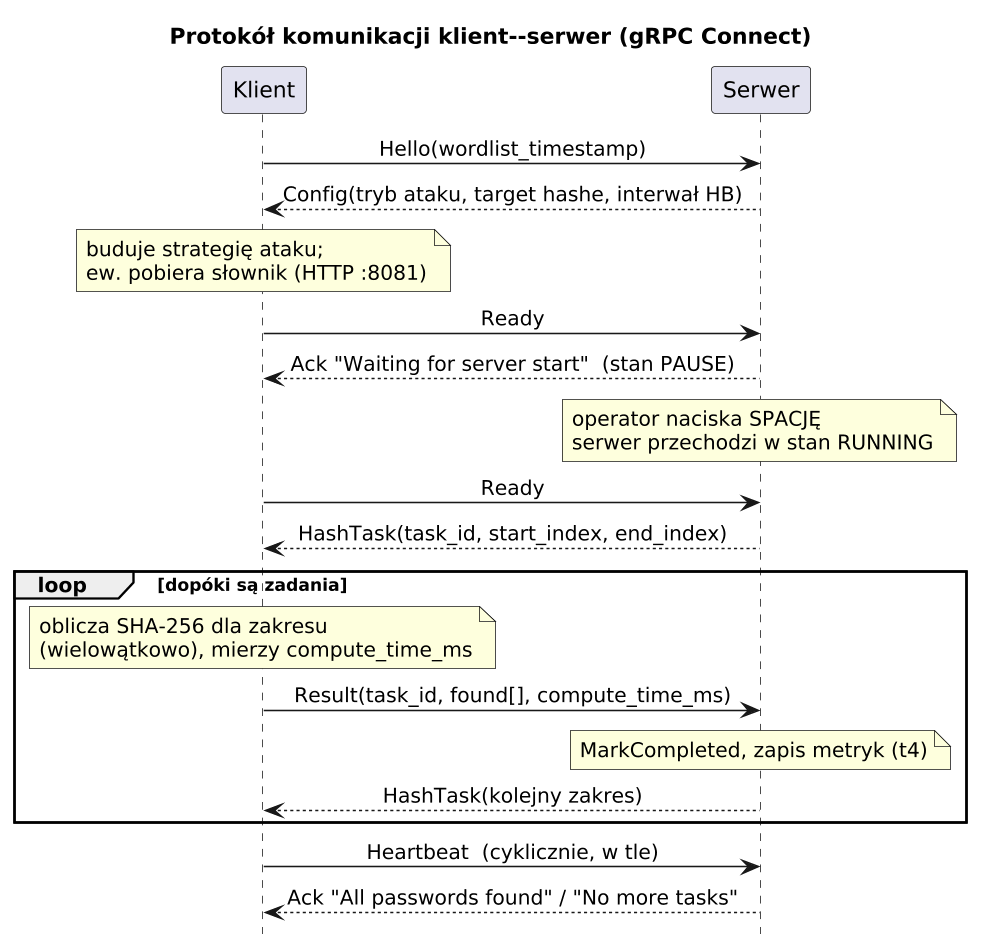
\includegraphics[width=0.92\linewidth,height=0.85\textheight,keepaspectratio]{diagramy/protokol.png}
\caption{Diagram sekwencji komunikacji klient--serwer w ramach jednego strumienia \texttt{Connect}.
Heartbeaty wysyłane są równolegle do głównej pętli pracy.}
\label{fig:seq}
\end{figure}

\subsection{Heartbeat, timeout i ponowny przydział}
Niezawodność systemu rozproszonego zapewniają trzy współpracujące mechanizmy:
\begin{itemize}
  \item \textbf{Heartbeat klienta}, \texttt{GrpcClient.HeartbeatLoop} cyklicznie (interwał z
        \texttt{Config}) wysyła pustą wiadomość \texttt{Heartbeat}; serwer aktualizuje
        ,,ostatnio widziany'' w \texttt{ClientTracker}.
  \item \textbf{Watchdog serwera}, dla każdego połączenia \texttt{PasswordBreakerService}
        uruchamia zadanie kontrolne; jeśli od klienta nie ma heartbeatu dłużej niż
        \texttt{HeartbeatTimeoutSeconds}, strumień zostaje zamknięty, a w \texttt{Cleanup}
        bieżące zadanie klienta wraca do kolejki (\texttt{MarkPending}).
  \item \textbf{Timeout zadania}, hostowana usługa \texttt{TaskTimeoutChecker} okresowo
        wywołuje \texttt{RequeueExpiredTasks}; zadanie pozostające w stanie \texttt{InProgress}
        dłużej niż \texttt{TaskTimeoutSeconds} jest zwracane do kolejki, co chroni przed
        zacięciem klienta na pojedynczej paczce.
\end{itemize}
Dodatkowo wynik dla zadania spoza aktywnego ,,przebiegu'' (lub już zakończonego) jest ignorowany;
identyfikator zadania i numer przebiegu (\texttt{RunSequence}) pełnią funkcję ochrony przed
duplikatami.

\subsection{Synchronizacja słownika}
W trybie słownikowym klient w wiadomości \texttt{Hello} przesyła znacznik czasu posiadanej kopii
słownika. Serwer w \texttt{Config} podaje znacznik aktualnej wersji. Jeśli znaczniki się różnią,
klient pobiera słownik zwykłym żądaniem HTTP GET z endpointu \texttt{/wordlist} (port 8081), po
czym ładuje go do pamięci. Dzięki temu wszystkie węzły operują na identycznym, uporządkowanym
zbiorze słów, co jest warunkiem poprawnego podziału zakresowego.

Dodatkowo serwer udostępnia osobną usługę \texttt{Monitor} (\texttt{Subscribe}), która
strumieniuje zdarzenia stanu systemu do opcjonalnego narzędzia podglądu.

% ==================================================================
\section{Jak ogólnie działa projekt}

\subsection{Cykl życia serwera i sterowanie przebiegiem}
Po uruchomieniu serwer wchodzi w stan \textbf{PAUSE}, klienci mogą się łączyć i pobierać
konfigurację, ale nie otrzymują zadań. Operator steruje przebiegiem z konsoli:
\begin{itemize}
  \item \textbf{SPACJA}, przełącza stan PAUSE\,$\leftrightarrow$\,RUNNING
        (\texttt{ServerRunState.Toggle}). Przejście w RUNNING otwiera nowy ,,przebieg
        eksperymentu'' (\texttt{ExperimentRunManager.StartNewRun}) i tworzy katalog wynikowy.
  \item \textbf{CTRL+C}, zatrzymuje serwer i zapisuje wyniki.
\end{itemize}
Każdy przebieg ma własny katalog \texttt{experiments/<nazwa>/} z plikami \texttt{metrics.csv}
i \texttt{results.csv}; nazwa koduje liczbę klientów, liczbę wątków, \texttt{ChunkSize} oraz
numer przebiegu, co ułatwia późniejszą analizę.

\subsection{Podział pracy na zadania}
\texttt{TaskManager} traktuje całą przestrzeń przeszukiwania jako uporządkowany zbiór
ponumerowanych kandydatów (\texttt{\_totalItems}). Przy każdym żądaniu \texttt{GetNextTask}
wycina kolejny zakres o szerokości \texttt{ChunkSize} (lub zwraca zadanie odzyskane z kolejki
\texttt{\_pendingTasks}, jeśli jakieś wróciło po błędzie). Zadanie przechodzi przez stany
przedstawione na rys.~\ref{fig:states}.

\begin{figure}[H]
\centering
\begin{tikzpicture}[node distance=22mm, font=\small]
  \node[comp, minimum width=24mm] (pend) {Pending};
  \node[comp, minimum width=24mm, right=34mm of pend] (prog) {InProgress};
  \node[comp, minimum width=24mm, right=34mm of prog] (done) {Completed};

  \draw[arr] (pend) -- node[above,font=\scriptsize]{GetNextTask} node[below,font=\scriptsize]{(przydział klientowi)} (prog);
  \draw[arr] (prog) -- node[above,font=\scriptsize]{MarkCompleted} node[below,font=\scriptsize]{(odebrano Result)} (done);
  \draw[arr] (prog) to[out=120,in=60] node[above,font=\scriptsize]{requeue: rozłączenie / timeout} (pend);
\end{tikzpicture}
\caption{Stany pojedynczego zadania w \texttt{TaskManager}. Zadanie zwrócone do kolejki trafia
ponownie do puli i może zostać przydzielone innemu klientowi.}
\label{fig:states}
\end{figure}

\subsection{Numerowanie kandydatów w trybie brute force}
\label{sec:bf-index}
Dla każdej długości hasła kombinacje numerowane są jak liczby w systemie pozycyjnym o podstawie
równej liczności alfabetu. Klient, otrzymawszy zakres indeksów \texttt{[start, end]}, wyznacza
długość i indeks lokalny, a następnie odtwarza kolejne hasła:

\begin{listing}[H]
\inputminted[firstline=184,lastline=196]{csharp}{../../password-break/password-break-client/HashWorker.cs}
\caption{Odtwarzanie hasła z indeksu, \texttt{HashWorker.IndexToPassword} (fragment pliku źródłowego).}
\end{listing}

\subsection{Obliczenia po stronie klienta (wielowątkowość)}
Po odebraniu \texttt{HashTask} klient dzieli przydzielony zakres na tyle podzakresów, ile wątków
ma do dyspozycji (\texttt{MaxDegreeOfParallelism}) i przetwarza je równolegle przez
\texttt{Parallel.ForEach}. Każdy wątek liczy SHA-256 kolejnych kandydatów i porównuje skrót ze
zbiorem \texttt{targetHashes}. Znalezione hasła trafiają do \texttt{ConcurrentBag}. Co pewną
liczbę iteracji sprawdzany jest token anulowania, dzięki czemu przerwanie połączenia szybko
zatrzymuje pracę.

\subsection{Pomiar metryk}
System mierzy czas zgodnie z założeniami z wczesnych etapów (znaczniki $t_1$--$t_4$):
\begin{itemize}
  \item klient mierzy \emph{czas obliczeń} $t_3-t_2$ (\texttt{Stopwatch} wokół \texttt{Process}),
  \item serwer zna czas wysłania zadania $t_1$ (\texttt{SentAtUtc}) i czas odbioru wyniku $t_4$,
  \item \emph{czas całkowity} $=t_4-t_1$, \emph{czas komunikacji} $=(t_4-t_1)-(t_3-t_2)$,
  \item \emph{przepustowość} $=$ liczba kandydatów $/$ czas obliczeń [kandydatów/s].
\end{itemize}
Klient mierzy czas właściwych obliczeń stoperem wokół wywołania strategii ataku:

\begin{listing}[H]
\inputminted[firstline=168,lastline=178]{csharp}{../../password-break/password-break-client/GrpcClient.cs}
\caption{Pomiar czasu obliczeń po stronie klienta (\texttt{GrpcClient.ProcessAndSendResult}).}
\end{listing}

\noindent a serwer po odebraniu wyniku wyznacza czasy całkowity, komunikacji i przepustowość:

\begin{listing}[H]
\inputminted[firstline=307,lastline=312]{csharp}{../../password-break/password-break-server/Services/PasswordBreakerService.cs}
\caption{Obliczanie metryk po stronie serwera (\texttt{PasswordBreakerService.SaveMetrics}).}
\end{listing}

Dla każdego ukończonego zadania serwer dopisuje wiersz do \texttt{metrics.csv},
m.in. \texttt{chunk\_size}, \texttt{client\_threads}, \texttt{connected\_clients\_at\_result},
\texttt{compute\_time\_ms}, \texttt{communication\_time\_ms}, \texttt{throughput\_candidates\_per\_sec}.
Mierzenie czasu całkowitego po stronie serwera eliminuje problem rozjazdu zegarów między maszynami.

% ==================================================================
\section{Metodologia eksperymentów i wyniki}

\subsection{Metodologia}
Przeprowadzono serię eksperymentów dla różnych liczb klientów oraz różnych wielkości chunków.
Aby sprawiedliwie porównywać konfiguracje o różnej liczbie klientów, wprowadzono pojęcie
\textbf{granulacji przypadającej na klienta}:
\[
\text{granulacja na klienta} \;=\; \frac{\text{rozmiar chunku}}{\text{liczba klientów}}.
\]
Każdy przebieg trwał ustalony czas, a liczbę klientów zwiększano do 14.

\subsection{Wpływ liczby klientów}
\begin{figure}[H]
\centering
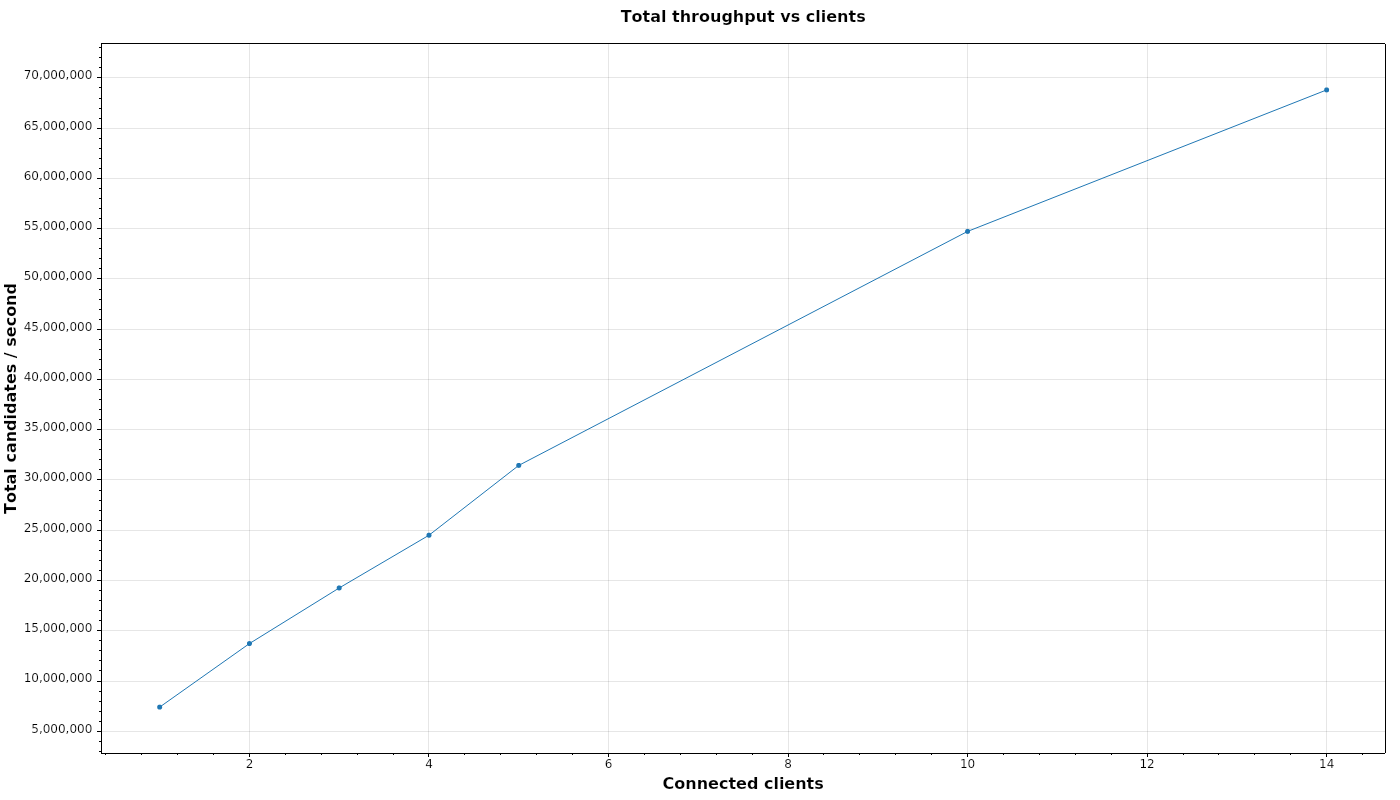
\includegraphics[width=0.86\linewidth]{wykresy/total_throughput_by_clients.png}
\caption{Całkowita przepustowość systemu w funkcji liczby podłączonych klientów.}
\label{fig:clients}
\end{figure}

\textbf{Obserwacje:} wraz ze wzrostem liczby klientów całkowita przepustowość rośnie niemal
liniowo; najwyższą wydajność uzyskano dla 14 klientów.

\textbf{Wniosek:} dodawanie kolejnych węzłów zwiększa wydajność, system wykorzystuje
równoległość obliczeń, a narzut koordynacji nie dominuje.

\subsection{Wpływ granulacji i liczby klientów}
\begin{figure}[H]
\centering
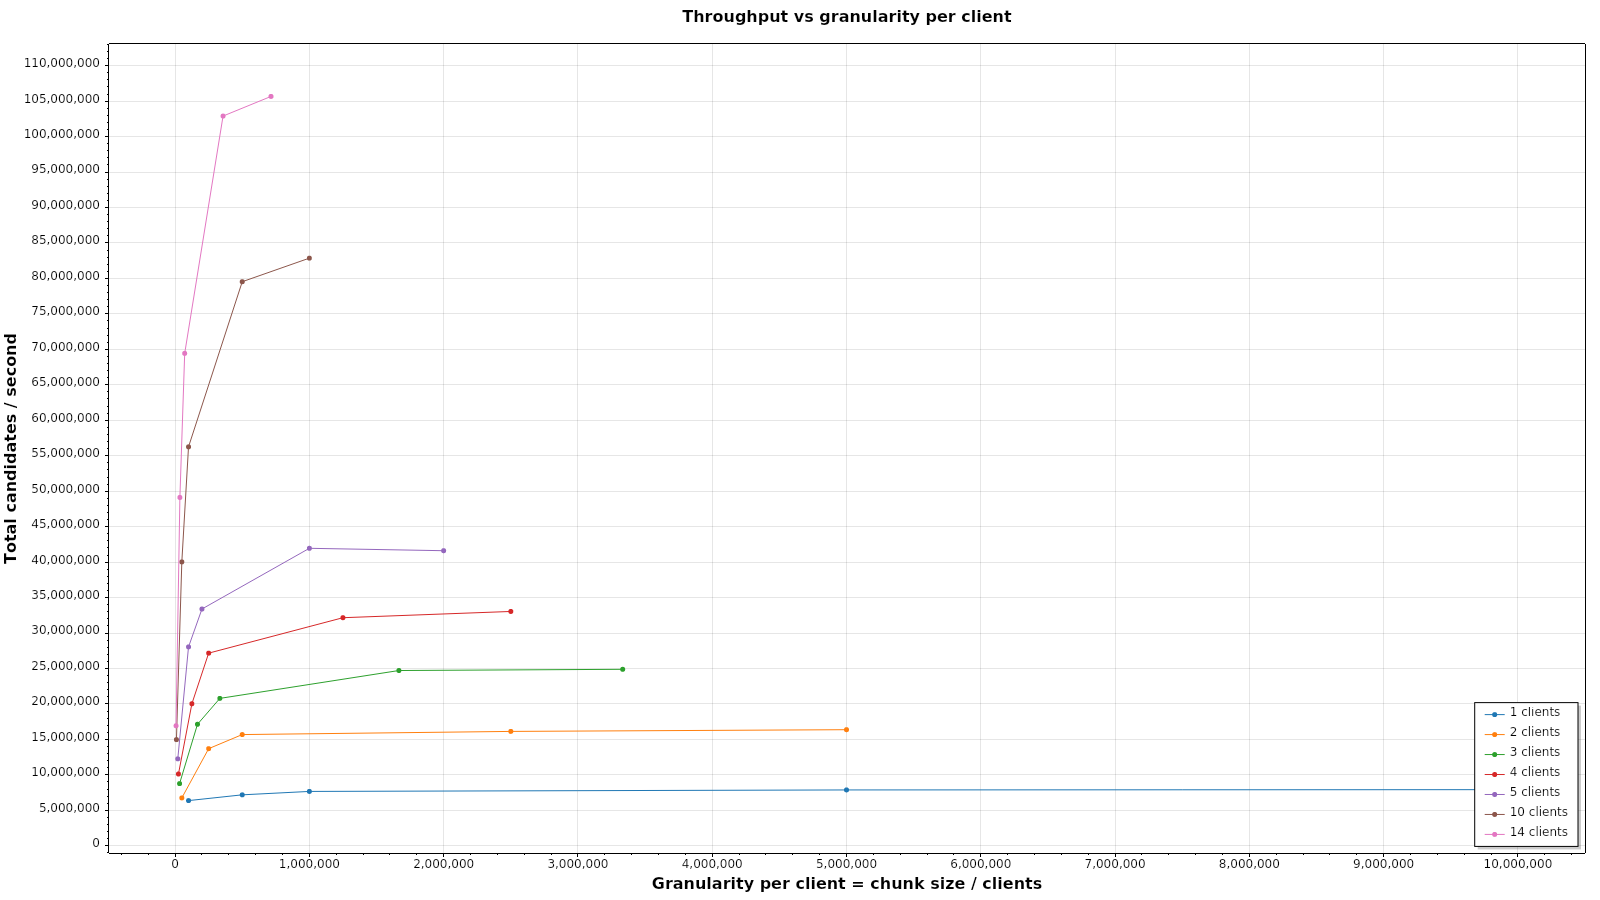
\includegraphics[width=0.92\linewidth]{wykresy/throughput_by_granularity_and_clients.png}
\caption{Przepustowość w funkcji granulacji przypadającej na klienta, dla różnych liczb klientów.}
\label{fig:gran}
\end{figure}

\textbf{Obserwacje:} dla małych chunków dominuje narzut komunikacyjny (częste wymiany
,,zadanie/wynik''), więc przepustowość jest niższa. Zwiększanie granulacji początkowo wyraźnie
podnosi wydajność, ale po przekroczeniu pewnego progu przyrost maleje (krzywa się wypłaszcza).
Dla większej liczby klientów osiągana jest wyższa przepustowość.

\textbf{Wniosek:} przy zbyt małej granulacji narzut komunikacji jest zbyt duży i obniża przepustowość.

\subsection{Łączny wpływ liczby klientów i granulacji}
Przepustowość i efektywność zależą jednocześnie od dwóch parametrów, liczby klientów oraz
wielkości chunku. Sama przepustowość rośnie monotonicznie z obu (co widać już na wykresach 2D),
więc bardziej pouczająca jest powierzchnia \emph{efektywności} $E(n)=S(n)/n$ (rys.~\ref{fig:effsurface}),
gdzie $x$ to liczba klientów, $y$ to wielkość chunku, a $z$ to efektywność.

\begin{figure}[H]
\centering
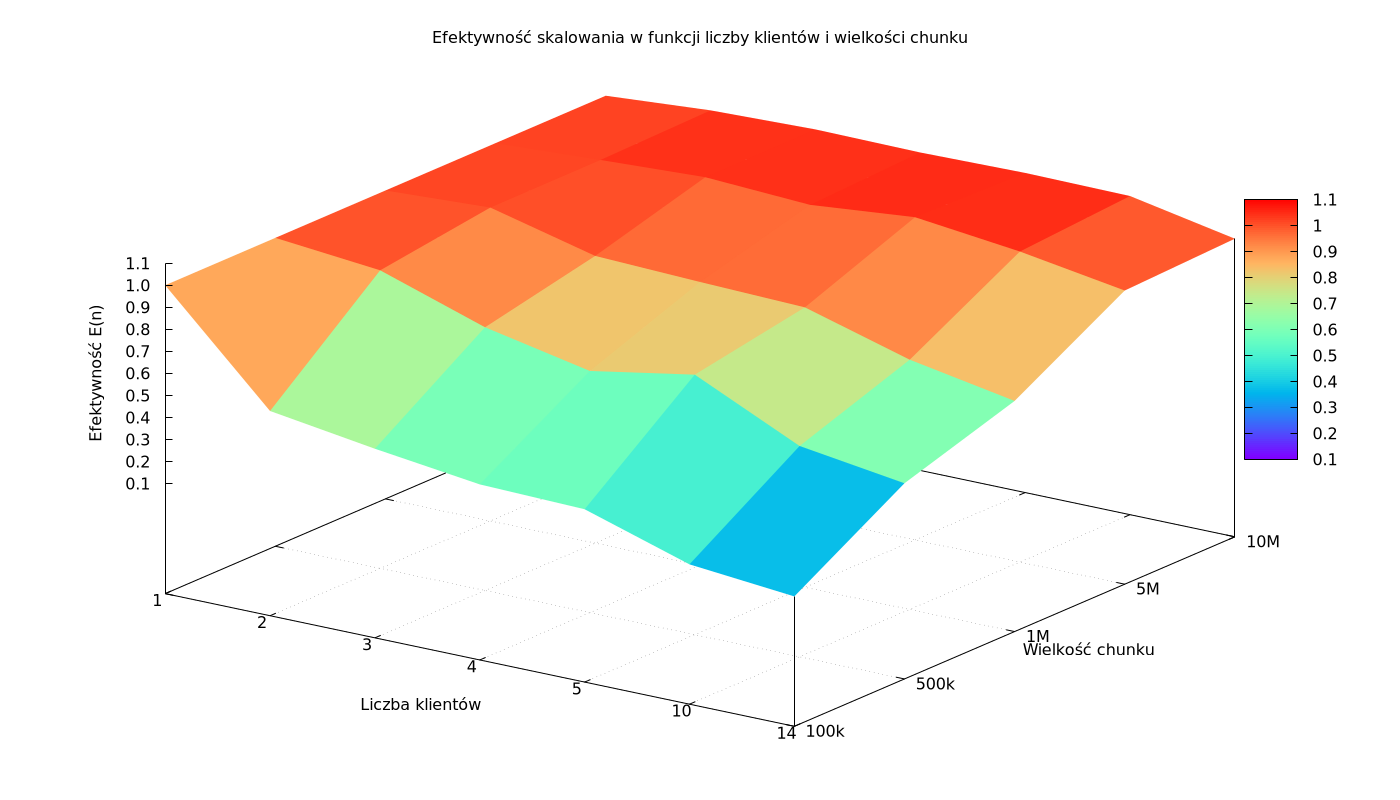
\includegraphics[width=0.92\linewidth]{wykresy/efficiency_surface.png}
\caption{Efektywność skalowania $E(n)=S(n)/n$ w funkcji liczby klientów i wielkości chunku.}
\label{fig:effsurface}
\end{figure}

\textbf{Obserwacje:} powierzchnia efektywności tworzy płaskowyż blisko 1{,}0 dla dużych chunków
(5M, 10M) niezależnie od liczby klientów oraz wyraźne ,,urwisko'' opadające do ok.~0{,}2 w narożniku
o małym chunku i dużej liczbie klientów.

\textbf{Wniosek:} oba czynniki działają łącznie, duża liczba klientów daje pełen efekt dopiero
przy odpowiednio dużej granulacji; sam wzrost liczby klientów przy małym chunku nie wystarcza.

\subsection{Przyspieszenie i efektywność skalowania}
\emph{Przyspieszenie} to iloraz całkowitej przepustowości dla $n$ klientów do przepustowości dla
jednego klienta (przy tej samej wielkości chunku), a \emph{efektywność} to przyspieszenie
znormalizowane liczbą klientów:
\[
S(n) = \frac{\text{przepustowość}(n)}{\text{przepustowość}(1)},
\qquad
E(n) = \frac{S(n)}{n}.
\]

\begin{figure}[H]
\centering
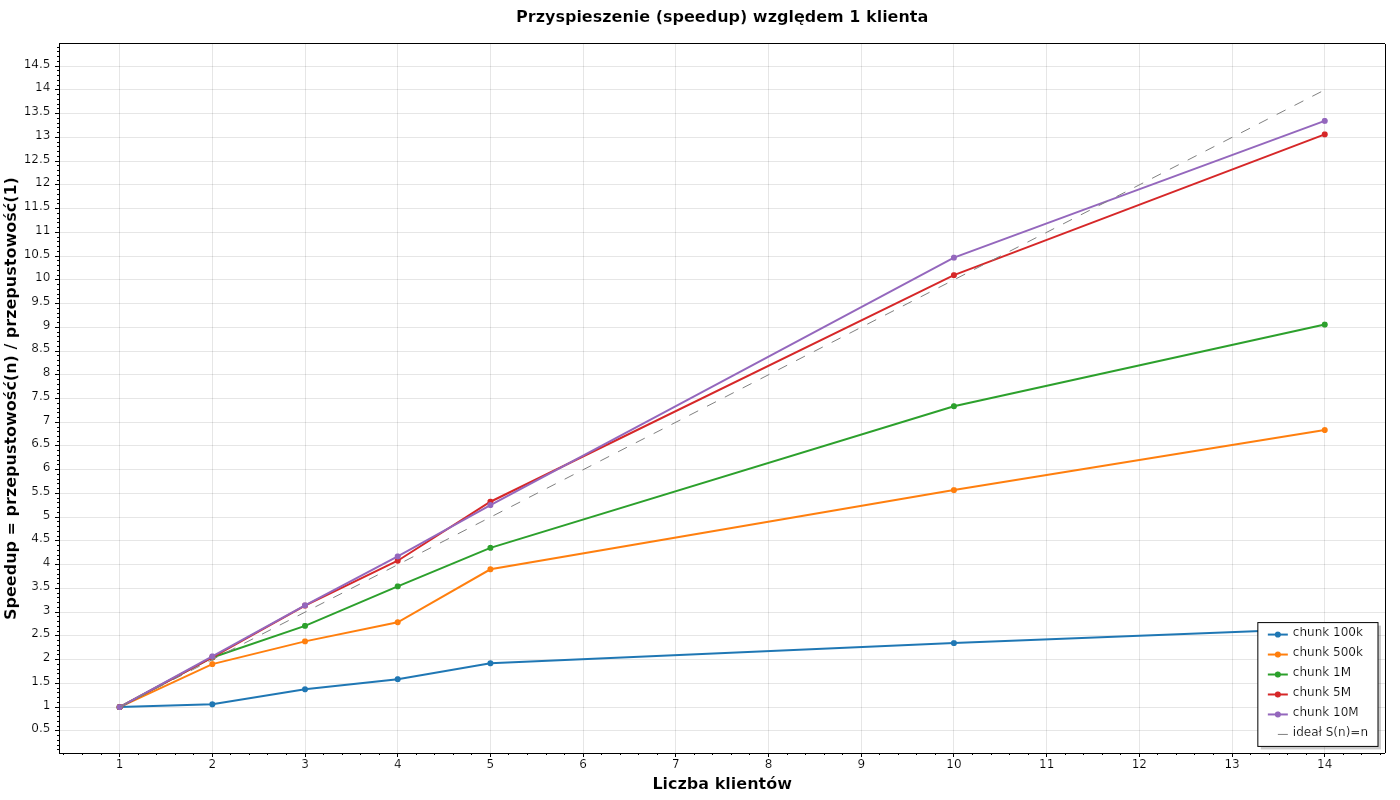
\includegraphics[width=0.82\linewidth]{wykresy/speedup_by_clients.png}
\caption{Przyspieszenie w funkcji liczby klientów, osobno dla każdej wielkości chunku.
Linia przerywana to skalowanie idealne $S(n)=n$.}
\label{fig:speedup}
\end{figure}

\begin{figure}[H]
\centering
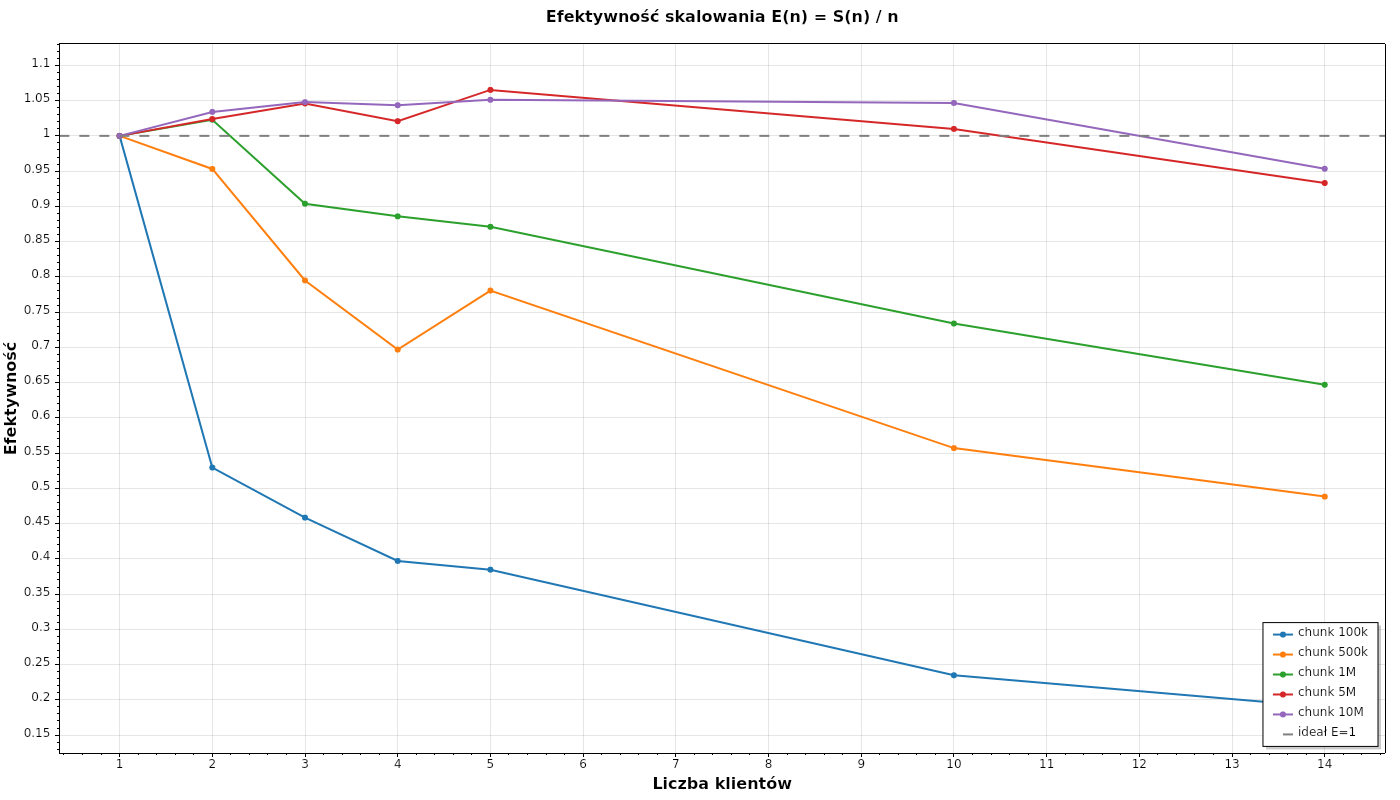
\includegraphics[width=0.82\linewidth]{wykresy/efficiency_by_clients.png}
\caption{Efektywność skalowania $E(n)=S(n)/n$. Wartość 1{,}0 oznacza skalowanie idealne.}
\label{fig:efficiency}
\end{figure}

\textbf{Obserwacje:} dla dużych chunków (5M, 10M) przyspieszenie pokrywa się z idealnym, a
efektywność utrzymuje się blisko 1{,}0 aż do 14 klientów (chwilami nieznacznie powyżej~1,
co wynika z wahań pomiaru i pełniejszego wykorzystania rdzeni). Dla małych chunków efektywność
gwałtownie spada, przy chunku 100k i 14 klientach wynosi ok.~0{,}2, bo system spędza czas na
obsłudze wielu drobnych zadań zamiast na obliczeniach.

\textbf{Wniosek:} system skaluje się niemal idealnie, pod warunkiem dostatecznie dużej granulacji.
Sama liczba klientów nie wystarcza, musi jej towarzyszyć odpowiednio duży chunk.

\subsection{Narzut komunikacji względem obliczeń}
Dla każdego zadania mierzony jest czas obliczeń (po stronie klienta) oraz czas komunikacji
($t_4-t_1$ pomniejszony o czas obliczeń, liczony na serwerze). Rysunek~\ref{fig:commabs}
zestawia oba czasy, a rysunek~\ref{fig:commfrac} pokazuje udział komunikacji w czasie obsługi
pojedynczego zadania.

\begin{figure}[H]
\centering
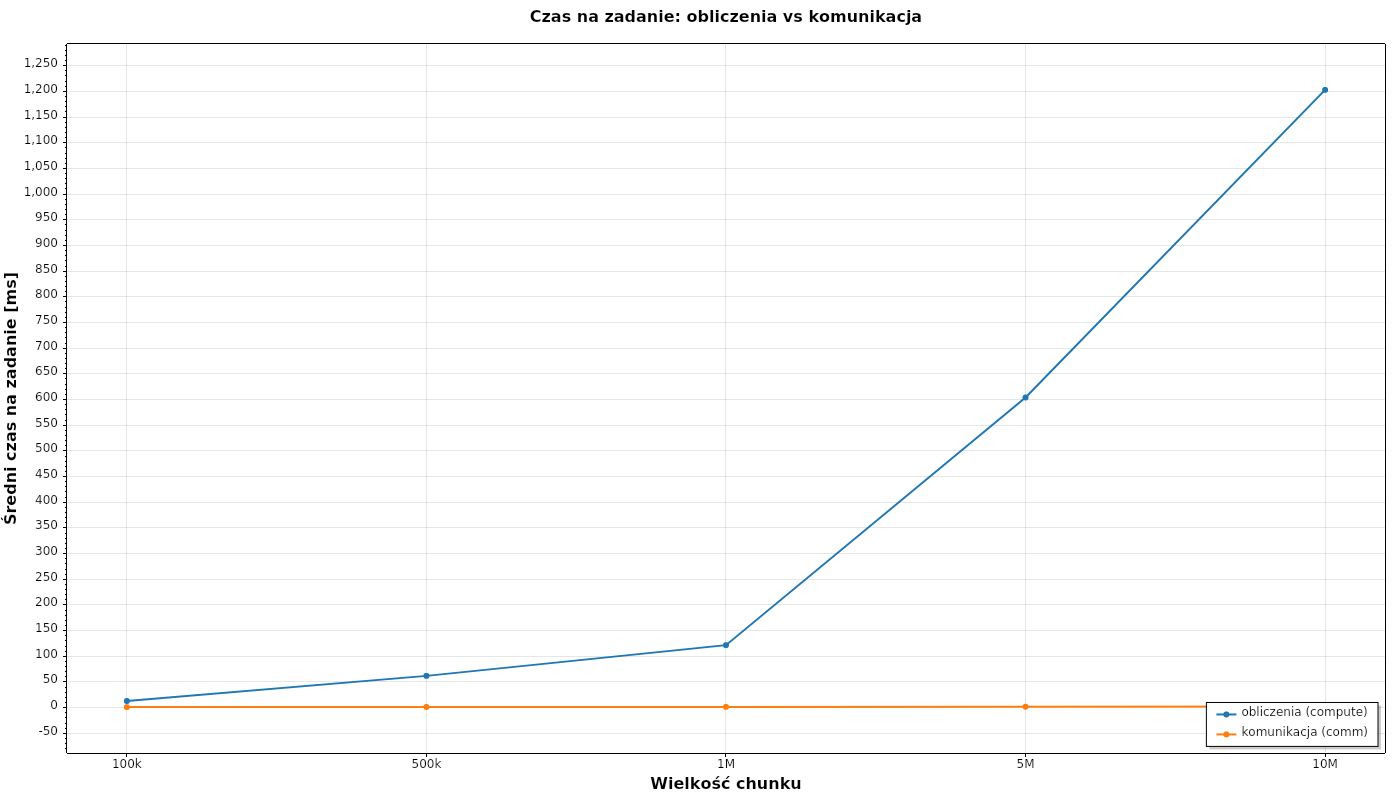
\includegraphics[width=0.82\linewidth]{wykresy/compute_vs_comm_by_chunk.png}
\caption{Średni czas obliczeń i komunikacji na jedno zadanie w funkcji wielkości chunku.}
\label{fig:commabs}
\end{figure}

\begin{figure}[H]
\centering
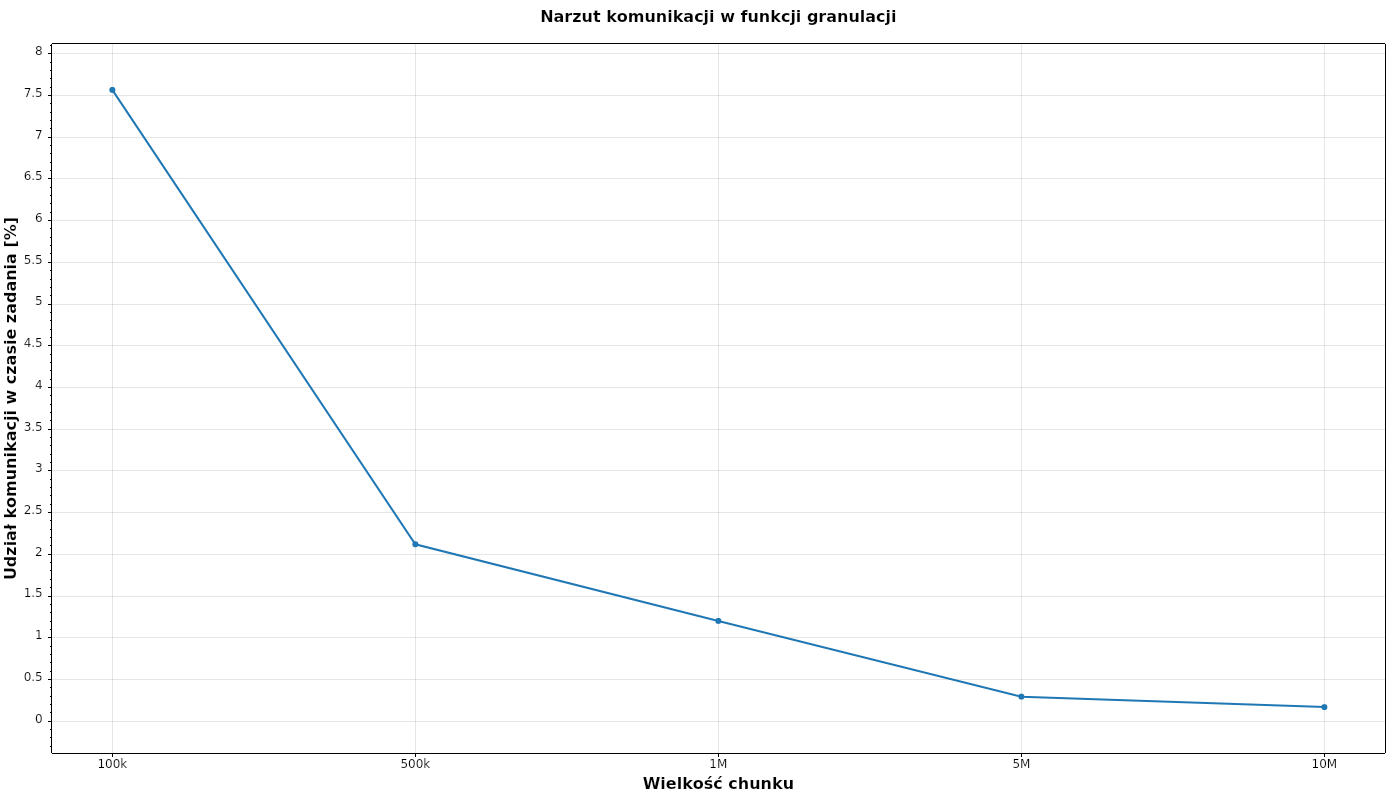
\includegraphics[width=0.82\linewidth]{wykresy/comm_overhead_by_chunk.png}
\caption{Udział czasu komunikacji w całkowitym czasie obsługi zadania.}
\label{fig:commfrac}
\end{figure}

\textbf{Obserwacje:} czas komunikacji jest niemal stały (ok.~1--2~ms na zadanie) i nie zależy od
wielkości chunku, natomiast czas obliczeń rośnie liniowo z chunkiem (od ok.~12~ms dla 100k do
ok.~1160~ms dla 10M). W rezultacie udział komunikacji spada z ok.~7{,}5\% dla chunku 100k do
poniżej~0{,}3\% dla chunku 10M.

\textbf{Wniosek:} narzut komunikacji jest stałym kosztem przypadającym na zadanie. Przy małych
chunkach jest ich bardzo wiele, więc ten koszt kumuluje się i obniża przepustowość; przy dużych
chunkach komunikacja jest pomijalna względem obliczeń. To spójne z obserwacjami dla granulacji
oraz z efektywnością skalowania.

\subsection{Balans obciążenia i stabilność połączeń}
Sprawdzono, czy praca rozkłada się równo i czy żaden węzeł nie odstawał. Pracę przypisano do
\emph{sesji klienta} (\texttt{client\_id}). Identyfikator sesji jest nadawany przy każdym
połączeniu (\texttt{Connect}), więc po rozłączeniu i ponownym podłączeniu klient otrzymuje nowy
\texttt{client\_id}; w zapisywanych metrykach nie ma stabilnego identyfikatora fizycznej maszyny.

\begin{figure}[H]
\centering
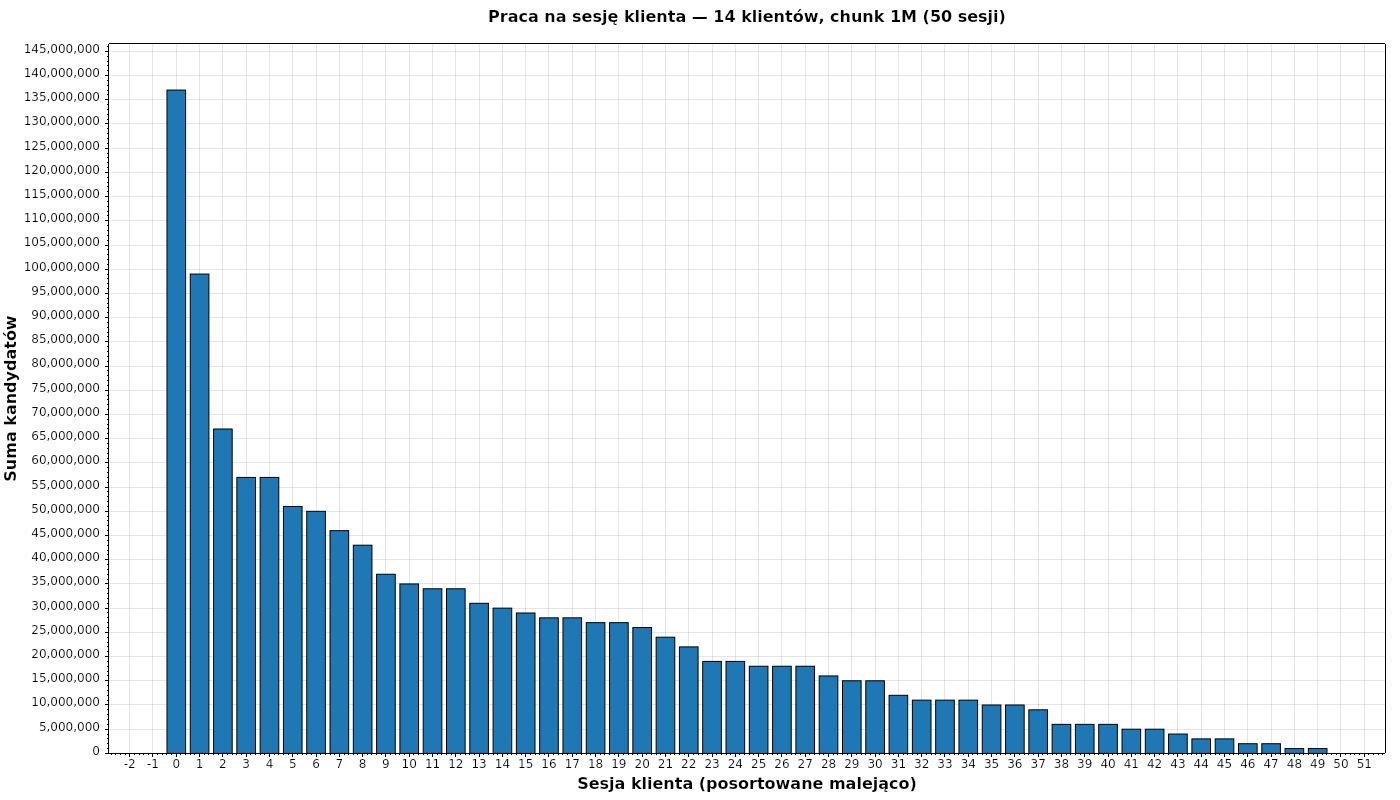
\includegraphics[width=0.82\linewidth]{wykresy/work_per_session_clients_14_chunk_1000000.png}
\caption{Rozkład pracy (sumy kandydatów) na sesję klienta dla przebiegu z 14 klientami i chunkiem 1M.}
\label{fig:worksession}
\end{figure}

\begin{figure}[H]
\centering
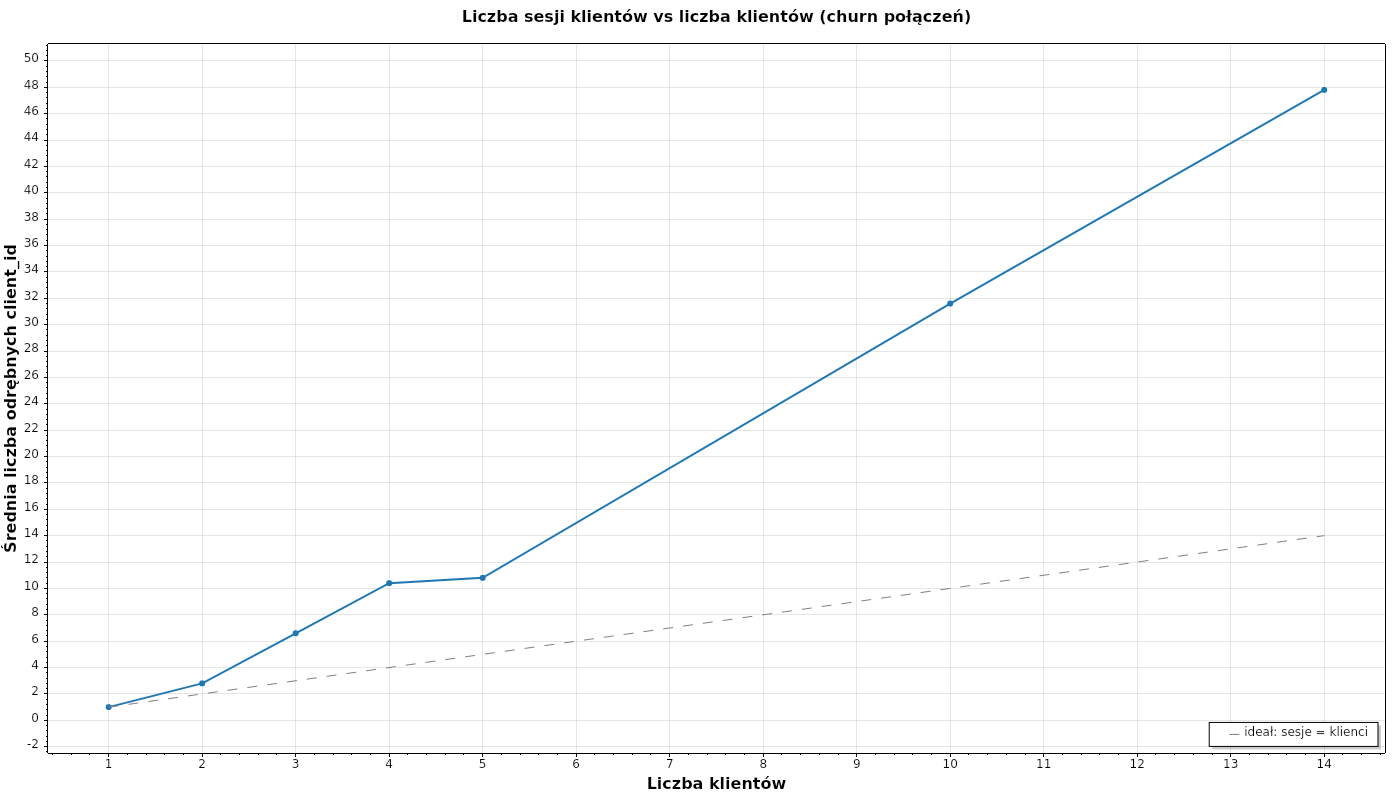
\includegraphics[width=0.82\linewidth]{wykresy/session_churn_by_clients.png}
\caption{Liczba odrębnych sesji (\texttt{client\_id}) względem zamierzonej liczby klientów.
Odstęp od linii idealnej to skala ponownych połączeń (churn).}
\label{fig:churn}
\end{figure}

\begin{figure}[H]
\centering
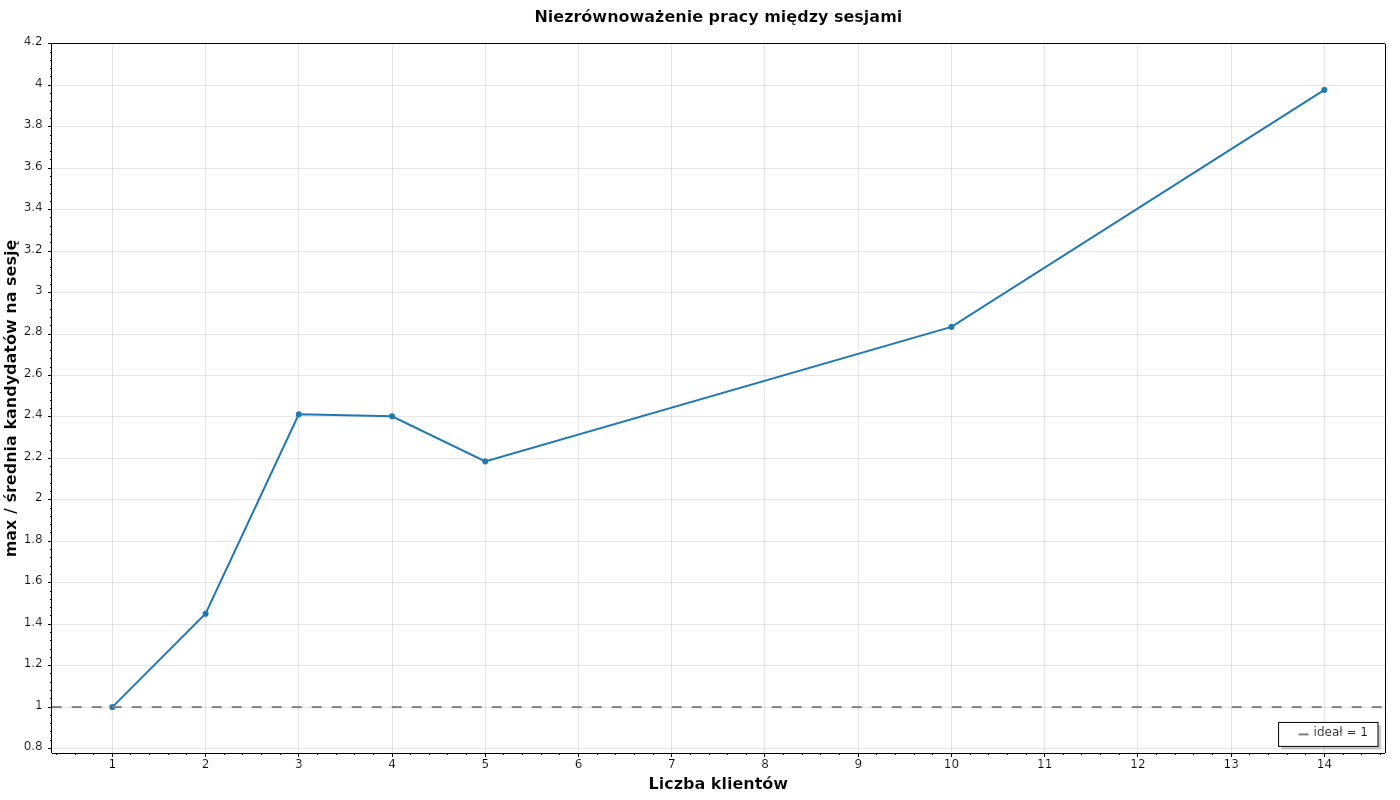
\includegraphics[width=0.82\linewidth]{wykresy/load_imbalance_by_clients.png}
\caption{Niezrównoważenie pracy: stosunek maksymalnej pracy sesji do średniej (1{,}0 = idealnie równo).}
\label{fig:imbalance}
\end{figure}

\textbf{Obserwacje:} dla małej liczby klientów (2--3) liczba sesji odpowiada liczbie klientów, a
praca rozkłada się dość równo. Przy większej liczbie klientów liczba sesji wyraźnie przewyższa
liczbę klientów (np.~14 klientów $\to$ ok.~50 sesji), co świadczy o licznych rozłączeniach i
ponownych połączeniach w trakcie przebiegu. To z kolei rozdrabnia pracę pojedynczej maszyny na
wiele krótkich sesji i podnosi pozorne niezrównoważenie (stosunek max/średnia rośnie do ok.~4
dla 14 klientów).

\textbf{Wniosek:} model \emph{pull} (klient sam pobiera kolejne zadania) sam w sobie wyrównuje
obciążenie, szybsze maszyny pobierają więcej pracy, więc żaden węzeł nie blokuje pozostałych.
Zaobserwowane niezrównoważenie wynika głównie z rozdrobnienia na sesje przy ponownych połączeniach,
a nie z faktu, że jakiś komputer ,,nie liczył''. Pełna analiza \emph{per maszyna} wymagałaby
zapisania stabilnego identyfikatora (np.~adresu IP klienta) w \texttt{metrics.csv}, obecnie
\texttt{client\_id} identyfikuje sesję, nie maszynę.

\subsection{Wcześniej zauważone problemy i ich usunięcie}
W trakcie prac (etap prototypu) zidentyfikowano i naprawiono ograniczenia wydajności:
\begin{itemize}
  \item rezygnacja z zapisywania \emph{wszystkich} generowanych skrótów (oszczędność pamięci),
  \item ograniczenie nadmiernego logowania w konsoli (mniejszy narzut),
  \item zwiększenie wykorzystania CPU dzięki wielowątkowemu przetwarzaniu zakresu po stronie
        klienta, tak aby dominował czas \emph{właściwych} obliczeń, a nie operacji pomocniczych.
\end{itemize}

% ==================================================================
\section{Wnioski końcowe}
\begin{itemize}
  \item Zbudowano działający system rozproszony w architekturze klient--serwer (gRPC, .NET),
        realizujący dynamiczny przydział pracy i zbieranie wyników.
  \item System \textbf{dobrze skaluje się} wraz ze wzrostem liczby klientów, przepustowość
        rośnie niemal liniowo, a dla dużych chunków efektywność skalowania utrzymuje się blisko
        1{,}0 aż do 14 klientów.
  \item \textbf{Granulacja zadań} ma istotny wpływ na wydajność: zbyt małe zadania powodują
        nadmierny narzut komunikacyjny, przez co przepustowość i efektywność spadają (przy chunku
        100k efektywność dla 14 klientów spada do ok.~0{,}2).
  \item \textbf{Narzut komunikacji jest stały}, ok.~1--2~ms na zadanie, niezależnie od wielkości
        chunku. O jego łącznym wpływie decyduje liczba zadań: udział komunikacji spada z ok.~7{,}5\%
        (chunk 100k) do poniżej~0{,}3\% (chunk 10M).
  \item \textbf{Obciążenie rozkłada się równomiernie} dzięki modelowi \emph{pull}; żaden węzeł nie
        blokował obliczeń. Per-sesyjne niezrównoważenie wynika z ponownych połączeń, a nie z
        nierównej pracy maszyn.
  \item Najlepsze wyniki osiągnięto przy dużej liczbie klientów.
  \item Mechanizmy heartbeat, watchdog i timeout zadań zapewniają odporność na rozłączenia i
        zawieszenia klientów, a numeracja przebiegów i zadań chroni przed duplikatami wyników.
  \item Czas właściwych obliczeń stanowi dominującą część czasu całkowitego, co potwierdza
        poprawność optymalizacji wykonanych w trakcie projektu.
\end{itemize}

\end{document}
